%
% simrecomb_docs.tex
%
% Copyright 2012 Darren Kessner
%
%   Licensed under the Apache License, Version 2.0 (the "License");
%   you may not use this file except in compliance with the License.
%   You may obtain a copy of the License at
%
%       http:%www.apache.org/licenses/LICENSE-2.0
%
%   Unless required by applicable law or agreed to in writing, software
%   distributed under the License is distributed on an "AS IS" BASIS,
%   WITHOUT WARRANTIES OR CONDITIONS OF ANY KIND, either express or implied.
%   See the License for the specific language governing permissions and
%   limitations under the License.
%

\documentclass{article}

\usepackage{graphicx}

% for 8.5 x 11 with pdflatex
\pdfpagewidth=\paperwidth 
\pdfpageheight=\paperheight


\begin{document}

\title{\texttt{simrecomb}}
\author{Darren Kessner}
\maketitle

%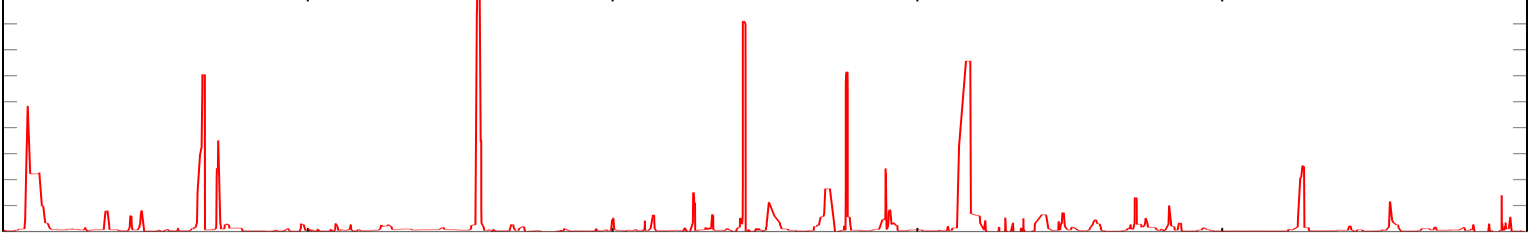
\includegraphics[width=1.0\textwidth]{fig/hotspots_bare.png}


\section*{Introduction}


\texttt{simrecomb} is a command-line program for simulating recombination and
admixture among multiple populations over multiple non-overlapping generations.
The user can specify population sizes, admixture rules for each population in
each generation, and genetic maps for recombination rates along chromosomes.
Individuals are diploid, and can have multiple chromosomes.  Individual
chromosome blocks are tracked during the course of the simulation, with
identifiers specifying the exact ancestral individual from which the block is
derived.

\begin{center}
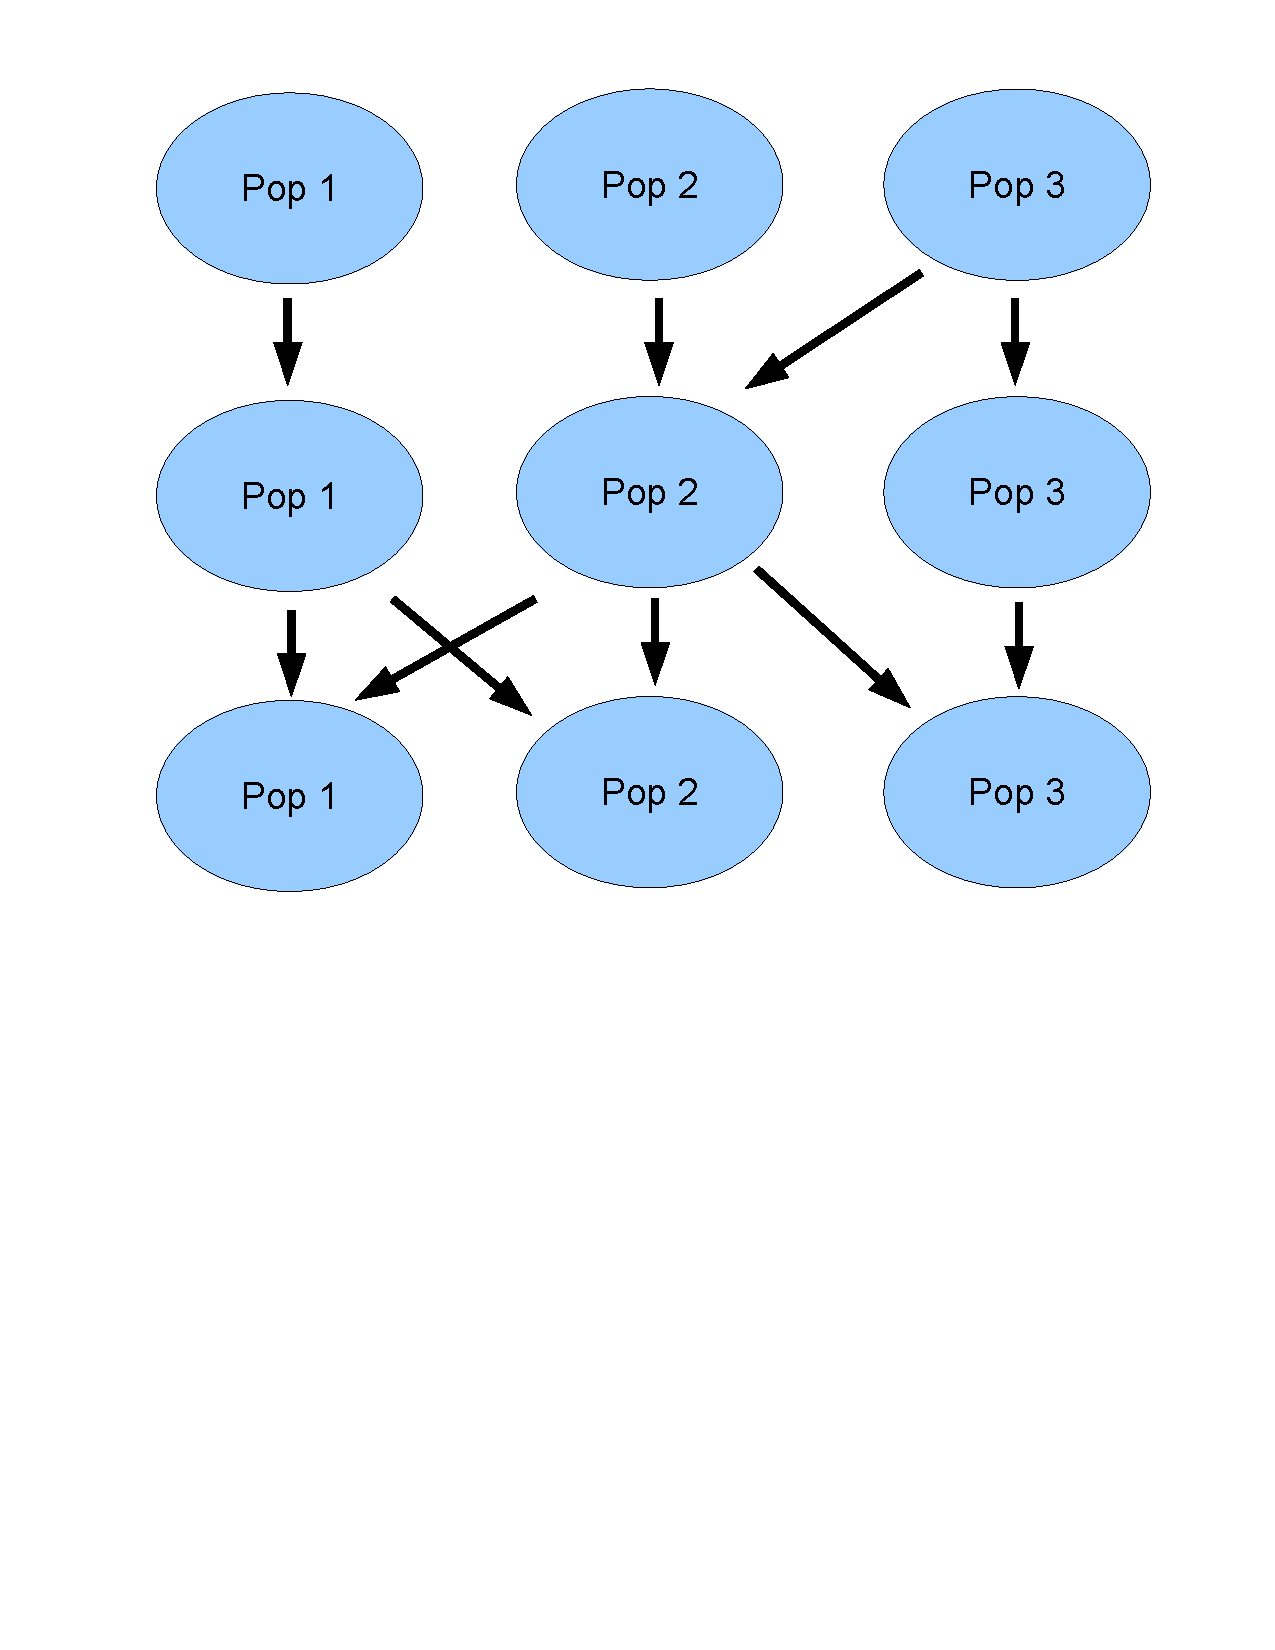
\includegraphics[width=.50\textwidth]{fig/simrecomb_cartoon.pdf}
\end{center}


\section*{Usage}
Running \texttt{simrecomb} with no arguments will output the usage string:
\begin{verbatim}
Usage: simrecomb <config_filename> <outputdir>
   or: simrecomb default (prints default config to stdout)
\end{verbatim}

\noindent The intended usage is to first create a boilerplate configuration file:
\begin{verbatim}
   simrecomb default > config.txt
\end{verbatim}

\noindent Then, edit \texttt{config.txt} and run the simulation:
\begin{verbatim}
   simrecomb config.txt outdir
\end{verbatim}
\noindent \texttt{simrecomb} will create a new directory named \texttt{outdir} and put
all output files there.

\section*{Configuration}

Here is an explanation of the default configuration file:

\begin{verbatim}
geneticMapFilenames 3
geneticMapFilename genetic_map_chr21_b36.txt
geneticMapFilename genetic_map_chr21_b36.txt
geneticMapFilename genetic_map_chr21_b36.txt
\end{verbatim}

\noindent These lines specify the genetic map file(s) -- in this case, it is
the same file, used for 3 chromosomes.  This genetic map file comes from the
HapMap project.

\begin{verbatim}
generation 0
population size=0 populationID=0
population size=10000 populationID=1 chromosomePairCount=3
population size=10000 populationID=2 chromosomePairCount=3
\end{verbatim}

\noindent Initial generation, with 3 populations, specified population sizes,
population ids, and number of chromosome pairs per individual.

\begin{verbatim}
generation 1
population size=10000 populationID=0 \\
    matingDistribution={<0.64|1,1><0.32|1,2><0.04|2,2>}
\end{verbatim}

\noindent Individuals in subsequent generations are created by drawing two
parents at random from the previous generation, according to a mating
distribution.  The line beginning \texttt{population} specifies admixture from
populations 1 and 2 in the previous generation 0, to create population 0 in
generation 1.  \texttt{matingDistribution} specifies the joint distribution of
the parent populations drawn to create individuals in this new population.  In
this case, 64\% both parents from pop1, 32\% one parent each from pop1 and
pop2, 4\% both parents from pop2 (equivalent to 80\% population 1, 20\%
population 2, with random mating).  Note: \textbackslash\textbackslash \,
indicates that the line has been split for the purposes of this documentation,
but is a single line in the file.

\begin{verbatim}
generation 2
population size=10000 populationID=0 matingDistribution={<1|0,0>}
\end{verbatim}

\noindent Create new population 0 from previous population 0, i.e. random mating.


\section*{Output}

\texttt{simrecomb} produces the following output files: \\

\noindent
\texttt{simrecomb\_config.txt}:  configuration used for the simulation \\
\texttt{log.txt}:  full log of the simulation \\
\texttt{pop?.txt}:  populations of the final generation \\

\noindent In the output data, each chromosome is listed on a separate
line, starting with + or -, which indicates which chromosome of the 
chromosome pair.  A blank line separates individuals. 
This is an example of a single chromosome:
\begin{verbatim}
+ { (0,<2,2127,0,1>) (14762956,<1,5503,0,0>) \\
    (15162040,<1,620,0,1>) (27852411,<1,8832,0,1>) }
\end{verbatim}

\noindent The chromosome above has 4 haplotype
blocks, starting at positions 0, 14762956, 15162040, 27852411.  The identity of
the first block is $\langle 2,2127,0,1 \rangle$, which indicates that it is from
population 2, individual 2127, 0th chromosome pair (0-based indexing),
chromosome 1 of the pair (here encoded \{0,1\} instead of +/-).


\section*{Subsampling populations}

\noindent Included with \texttt{simrecomb} is a tool for subsampling from the
final populations: \texttt{subsample\_population}.  Running
\texttt{subsample\_population} with no arguments will give the usage
information. \\


\section*{Combining \texttt{simrecomb} with \texttt{ms}}

(Currently this works for the case of a final population resulting from
admixture of populations 1 and 2 only -- email Darren if you would like
to handle a more general case.) \\

\noindent The tool \texttt{recombine\_data} (packaged with \texttt{simrecomb}) can be
used to combine the output from \texttt{simrecomb} with the output from Richard
Hudson's \texttt{ms} tool. \\

\noindent \texttt{recombine\_data} maps the 0/1 SNP values in \texttt{ms} format to
chromosomes in ancestral populations 1 and 2.  Individuals in the final
generation have chromosomes that are mosaics of haplotype blocks from the two
ancestral populations.  \texttt{recombine\_data} outputs sequences for these
mosaic chromosomes. \\

\noindent Running \texttt{recombine\_data} with no arguments will give the
usage information. \\



\end{document}


